% =============================================================================
% EXPERIMENTS - CITA Paper in ALKALI Format
% =============================================================================

\vspace{-2mm}
\section{Experiments}
\label{sec:experiments}

We present our experimental setup, including the training pipeline, model variants, evaluation benchmarks, hyperparameter optimization, and training dynamics.

\vspace{-2mm}
\subsection{Training Pipeline}
\label{sec:training_pipeline_exp}

Following the staged approach from Section~\ref{sec:training_pipeline}, we train on PKU-SafeRLHF~\cite{ji2024pku,bai2022training} using an NVIDIA A100-40GB GPU with LoRA~\cite{hu2022lora} adapters. Training proceeds through four stages:

\begin{enumerate}[leftmargin=*,itemsep=1pt]
    \item \textbf{Base}: Llama-3.1-8B~\cite{dubey2024llama} (pretrained weights)
    \item \textbf{SFT}: Fine-tune on PKU chosen responses
    \item \textbf{DPO}: Train on PKU preference pairs
    \item \textbf{CITA}: Add instruction-conditioning with mandatory KL
\end{enumerate}

\begin{figure*}[t]
\centering
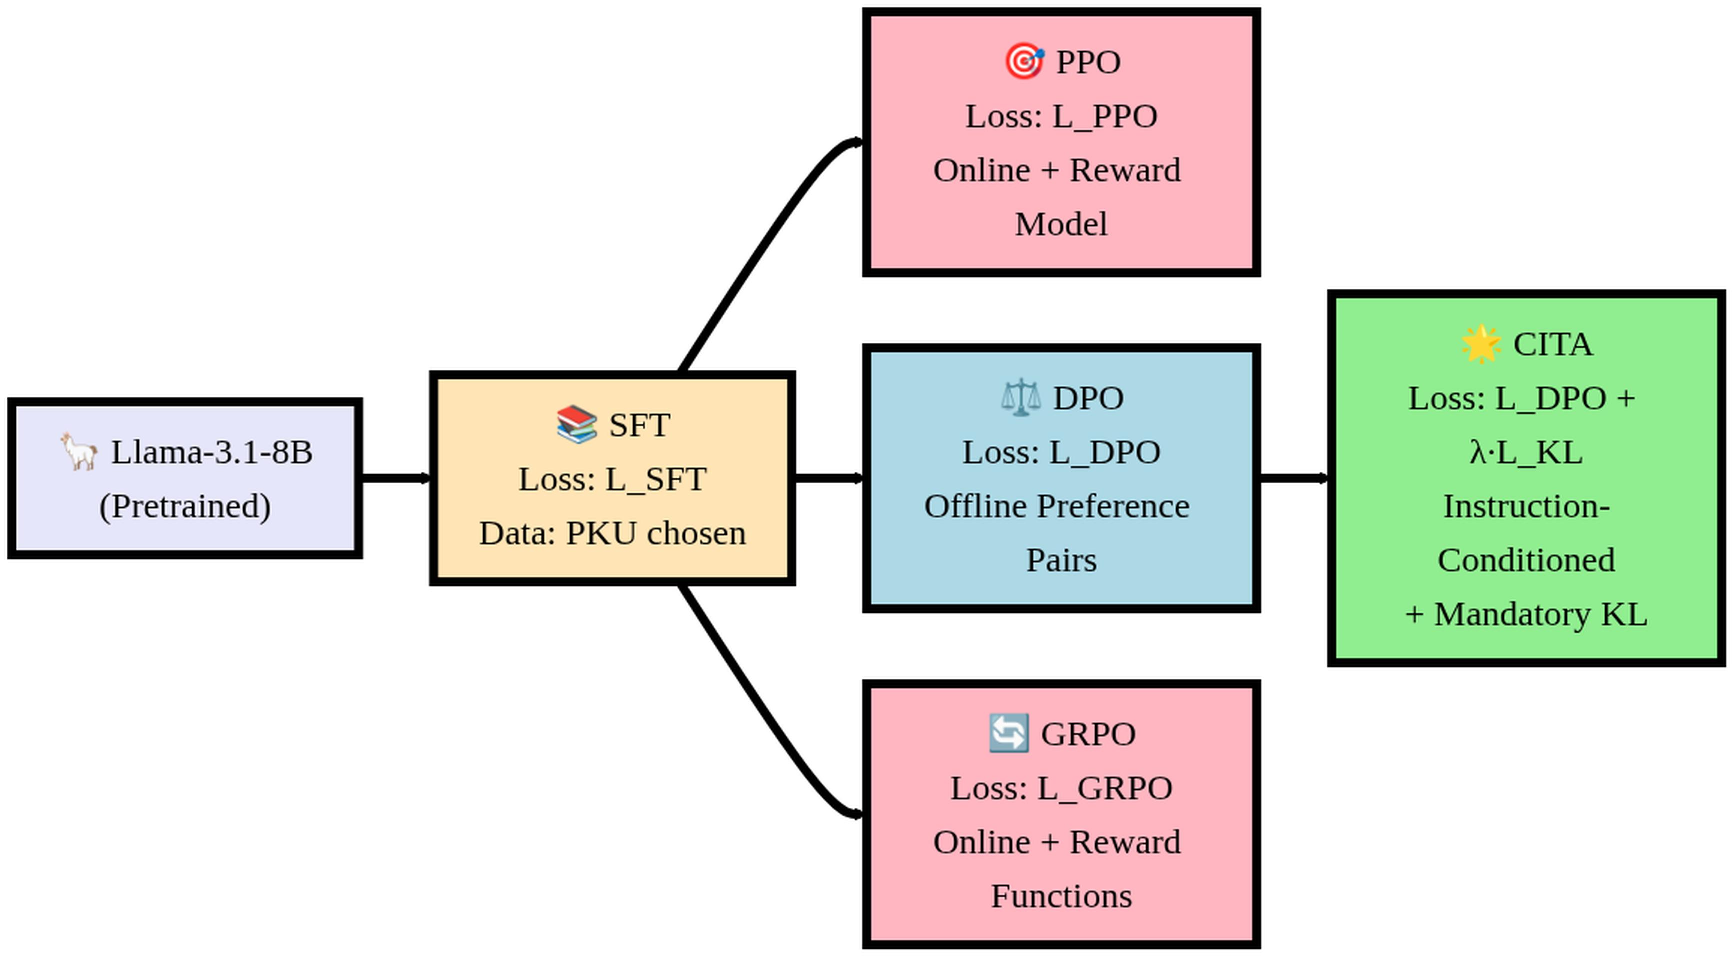
\includegraphics[width=0.9\textwidth]{figures/pipeline/training_pipeline.pdf}
\caption{\textbf{Training Pipeline}: All methods branch from SFT. PPO and GRPO are online methods requiring reward model/functions. DPO uses offline preference pairs. CITA stacks on DPO with instruction-conditioning and mandatory KL regularization.}
\label{fig:training_pipeline}
\vspace{-3mm}
\end{figure*}

\vspace{-2mm}
\subsection{Model Variants}
\label{sec:model_variants}

We train 10 model variants across 5 methods (SFT, PPO, GRPO, DPO, CITA) $\times$ 2 instruction settings (NoInstruct, Instruct):

\begin{table}[H]
\centering
\footnotesize
\begin{tabular}{@{}lll@{}}
\toprule
\textbf{Model} & \textbf{Training Path} & \textbf{Instruction} \\
\midrule
SFT\_NI & Base$\rightarrow$SFT & No \\
\hline
SFT\_I & Base$\rightarrow$SFT & Yes \\
\hline
PPO\_NI & Base$\rightarrow$SFT$\rightarrow$PPO & No \\
\hline
PPO\_I & Base$\rightarrow$SFT$\rightarrow$PPO & Yes \\
\hline
GRPO\_NI & Base$\rightarrow$SFT$\rightarrow$GRPO & No \\
\hline
GRPO\_I & Base$\rightarrow$SFT$\rightarrow$GRPO & Yes \\
\hline
DPO\_NI & Base$\rightarrow$SFT$\rightarrow$DPO & No \\
\hline
DPO\_I & Base$\rightarrow$SFT$\rightarrow$DPO & Yes \\
\hline
CITA\_NI & Base$\rightarrow$SFT$\rightarrow$DPO$\rightarrow$CITA & No \\
\hline
CITA\_I & Base$\rightarrow$SFT$\rightarrow$DPO$\rightarrow$CITA & Yes \\
\bottomrule
\end{tabular}
\caption{10 model variants. NI = NoInstruct (standard prompts), I = Instruct (with behavioral instructions). PPO, GRPO, DPO branch from SFT; CITA stacks on DPO.}
\label{tab:model_variants}
\vspace{-4mm}
\end{table}

\textbf{Comparison Design.} By evaluating NoInstruct vs. Instruct variants, we measure each method's \textit{instruction sensitivity}---the improvement from adding alignment instructions.

\vspace{-2mm}
\subsection{Evaluation Benchmarks}
\label{sec:benchmarks}

We evaluate on 5 benchmarks with deterministic metrics (no LLM-as-judge):

\begin{table}[H]
\centering
\footnotesize
\begin{tabularx}{\columnwidth}{@{}lXX@{}}
\toprule
\textbf{Benchmark} & \textbf{Cases} & \textbf{Instr. Types} \\
\midrule
ISD (ours) & 3,000 & 10 types \\
\hline
TruthfulQA & 1,634 & HON/CONF \\
\hline
Cond. Safety & 1,000 & STRICT/PERMIS. \\
\hline
Length Control & 1,000 & CONC./DETAIL. \\
\hline
AQI & 2,800 & 7 axioms \\
\bottomrule
\end{tabularx}
\caption{Evaluation benchmarks. All use deterministic metrics.}
\label{tab:benchmarks}
\vspace{-4mm}
\end{table}

\paragraph{Metrics.}

\begin{table}[H]
\centering
\footnotesize
\begin{tabular}{@{}ll@{}}
\toprule
\textbf{Benchmark} & \textbf{Metric (Ideal Value)} \\
\midrule
ISD & Fidelity $\times$ Behavioral Shift (1.0) \\
\hline
TruthfulQA & HON $-$ CONF uncertainty difference (+) \\
\hline
Conditional Safety & $|$STRICT $-$ PERMISSIVE$|$ (1.0) \\
\hline
Length Control & DETAILED/CONCISE word ratio ($>$4) \\
\hline
AQI & (CHI + XB) / 2 clustering score (100) \\
\bottomrule
\end{tabular}
\caption{Metric definitions. Higher is better for all except TruthfulQA (positive direction matters).}
\label{tab:metrics}
\vspace{-4mm}
\end{table}

\textbf{ISD Types}: Neutral, Conservative, Liberal, Regulatory, Empathetic, Safety, Educational, Concise, Professional, Creative.

\textbf{AQI Axioms}: Civility, Duty, Empathy, Information, Justice, Well-being, Wisdom.

\vspace{-2mm}
\subsection{Hyperparameter Optimization}
\label{sec:hyperparams}

We use Optuna~\cite{akiba2019optuna} with TPE sampler (12 trials) to optimize hyperparameters, following best practices from hyperparameter optimization literature~\cite{liang2023holistic}. Key finding: \textbf{CITA\_Instruct requires $\sim$50\% lower learning rate} than CITA\_NoInstruct because instruction-augmented sequences are 30--40\% longer, causing larger gradients.

\begin{table}[H]
\centering
\footnotesize
\begin{tabular}{@{}lcc@{}}
\toprule
\textbf{Hyperparameter} & \textbf{NoInstruct (T5)} & \textbf{Instruct (T7)} \\
\midrule
Learning rate & 6.83e-6 & 5.41e-6 \\
\hline
$\lambda_{\text{KL}}$ & 0.00052 & 0.00023 \\
\hline
$\beta$ (DPO temp.) & 0.119 & 0.107 \\
\hline
Weight decay & 0.0091 & 0.0109 \\
\hline
Warmup ratio & 7.5\% & 10.0\% \\
\midrule
Final margin & 6.95 & 7.52 \\
\hline
Accuracy & 89.5\% & 89.0\% \\
\bottomrule
\end{tabular}
\caption{Optimal hyperparameters from Optuna search. T5/T7 = trial number of best configuration.}
\label{tab:hyperparams}
\vspace{-4mm}
\end{table}

\vspace{-2mm}
\subsection{Training Dynamics}
\label{sec:training_dynamics}

We analyze key training curves across all alignment methods.

\begin{figure*}[t]
\centering
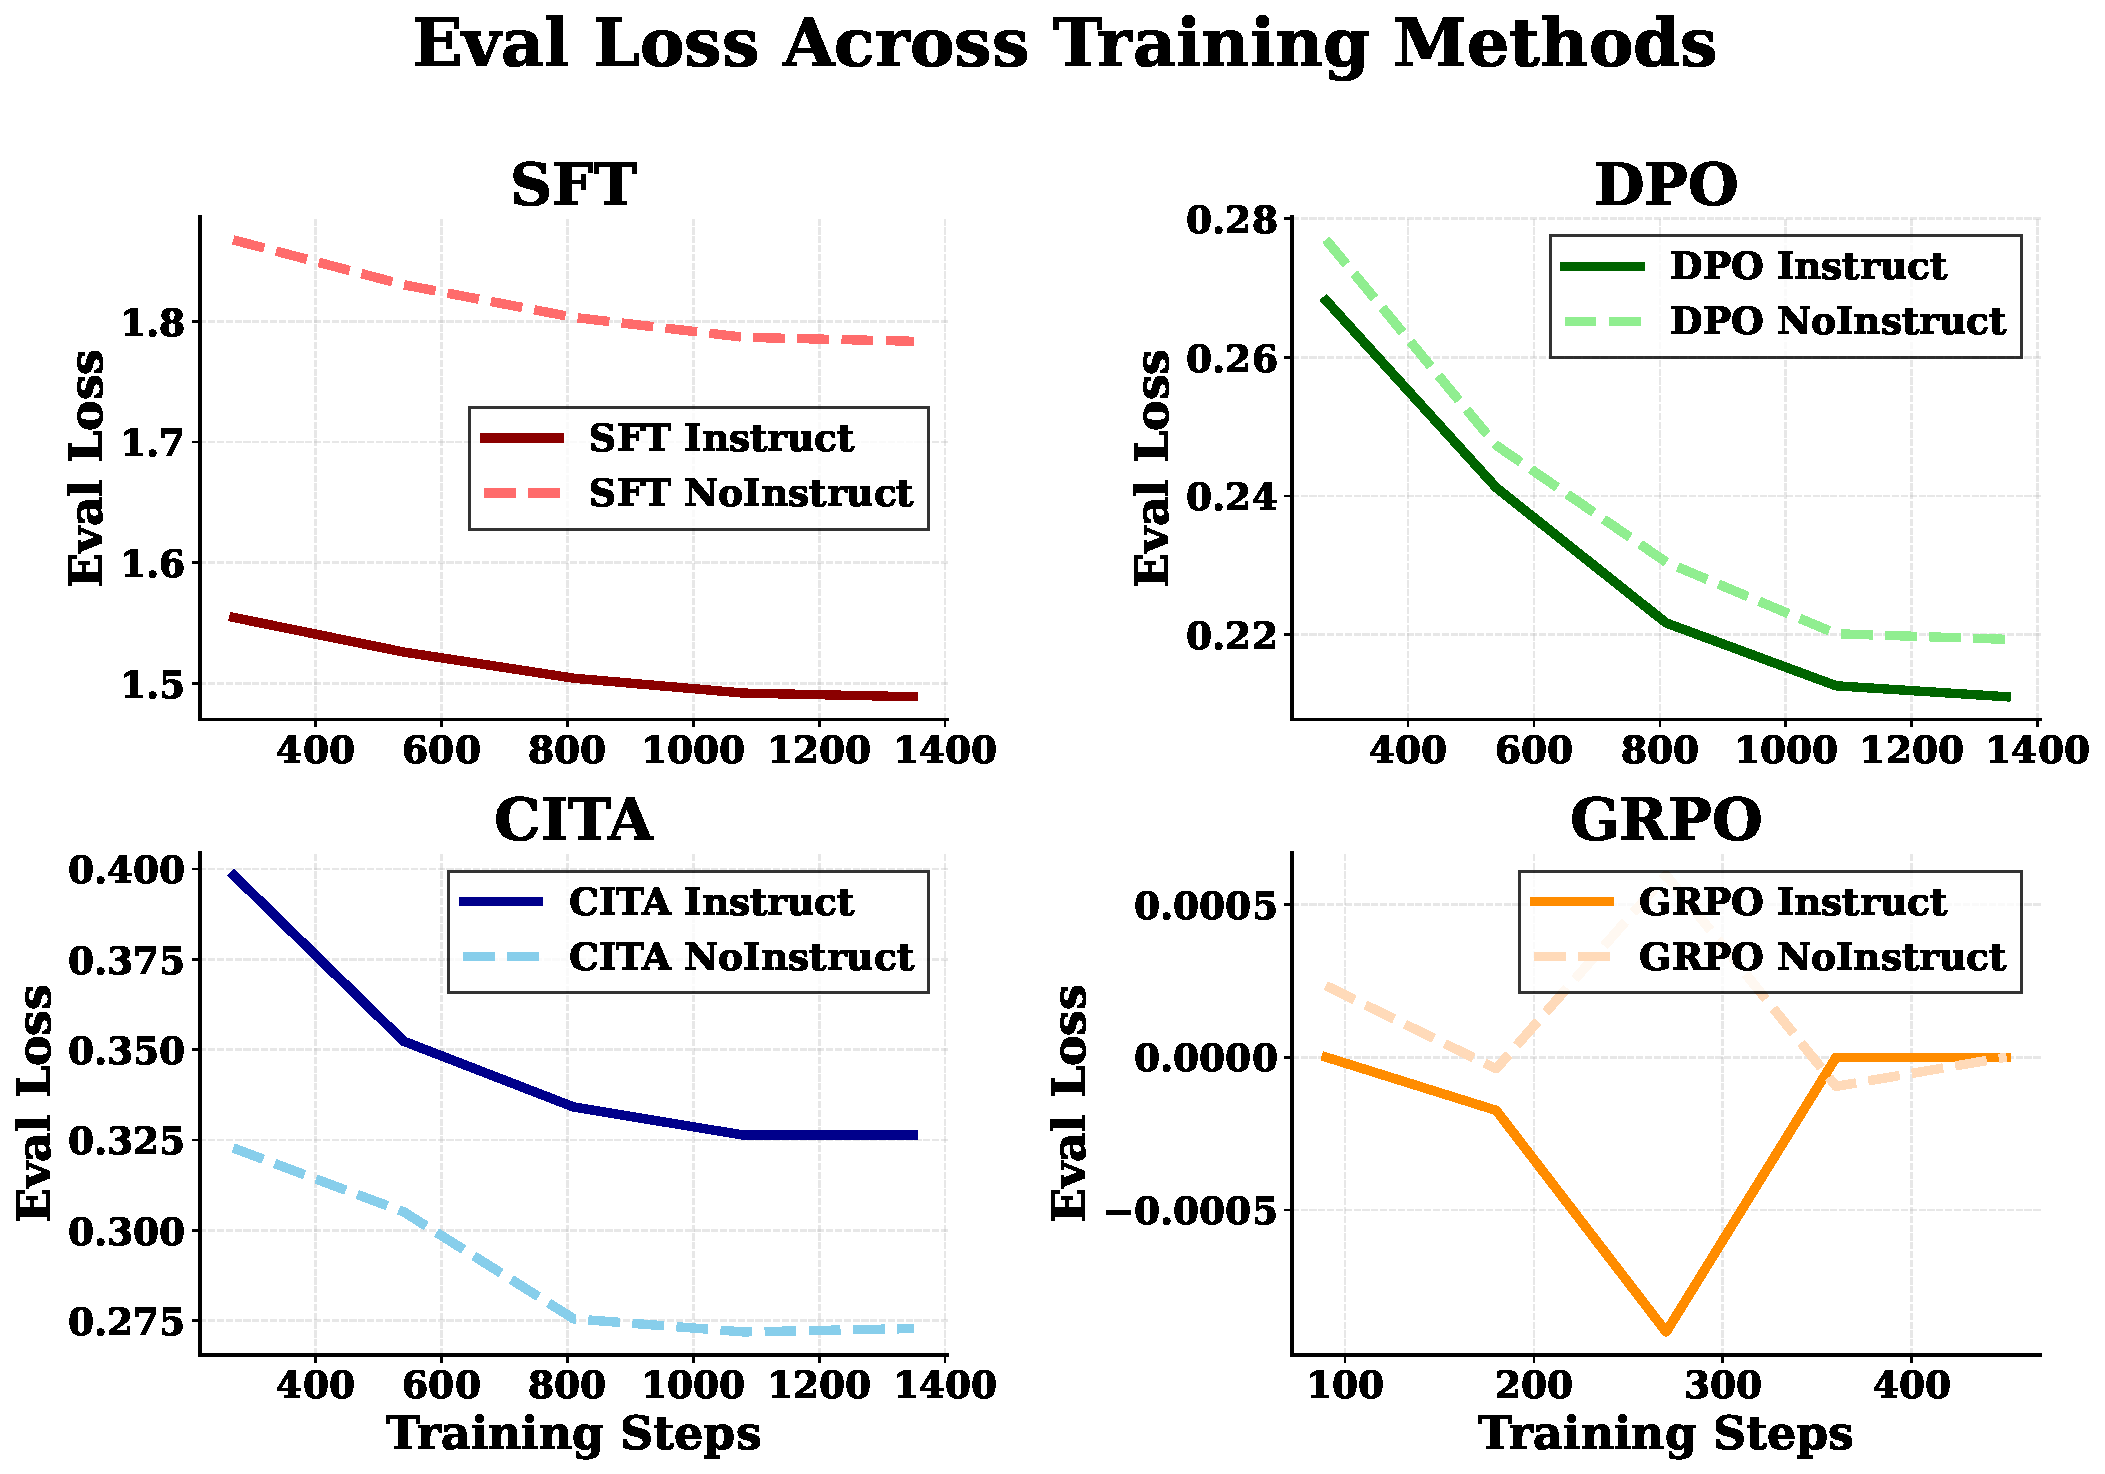
\includegraphics[width=0.9\textwidth]{figures/training/combined_eval_loss.pdf}
\caption{\textbf{Eval Loss Across Training Methods}: 2$\times$2 subplot showing eval loss for all 4 trainer types with independent y-axes (necessary due to vastly different loss scales). \textbf{SFT} (top-left): Loss $\sim$1.5--1.9, Instruct converges lower. \textbf{DPO} (top-right): Loss $\sim$0.21--0.28, smooth convergence. \textbf{CITA} (bottom-left): Loss $\sim$0.27--0.40, NoInstruct converges lower but CITA\_Instruct achieves better reward margins. \textbf{GRPO} (bottom-right): Loss oscillates near zero ($\pm$0.001), characteristic of online RL training dynamics. Note: PPO tensorboard logs were empty (TRL logging issue).}
\label{fig:training_loss}
\vspace{-3mm}
\end{figure*}

\begin{figure*}[t]
\centering
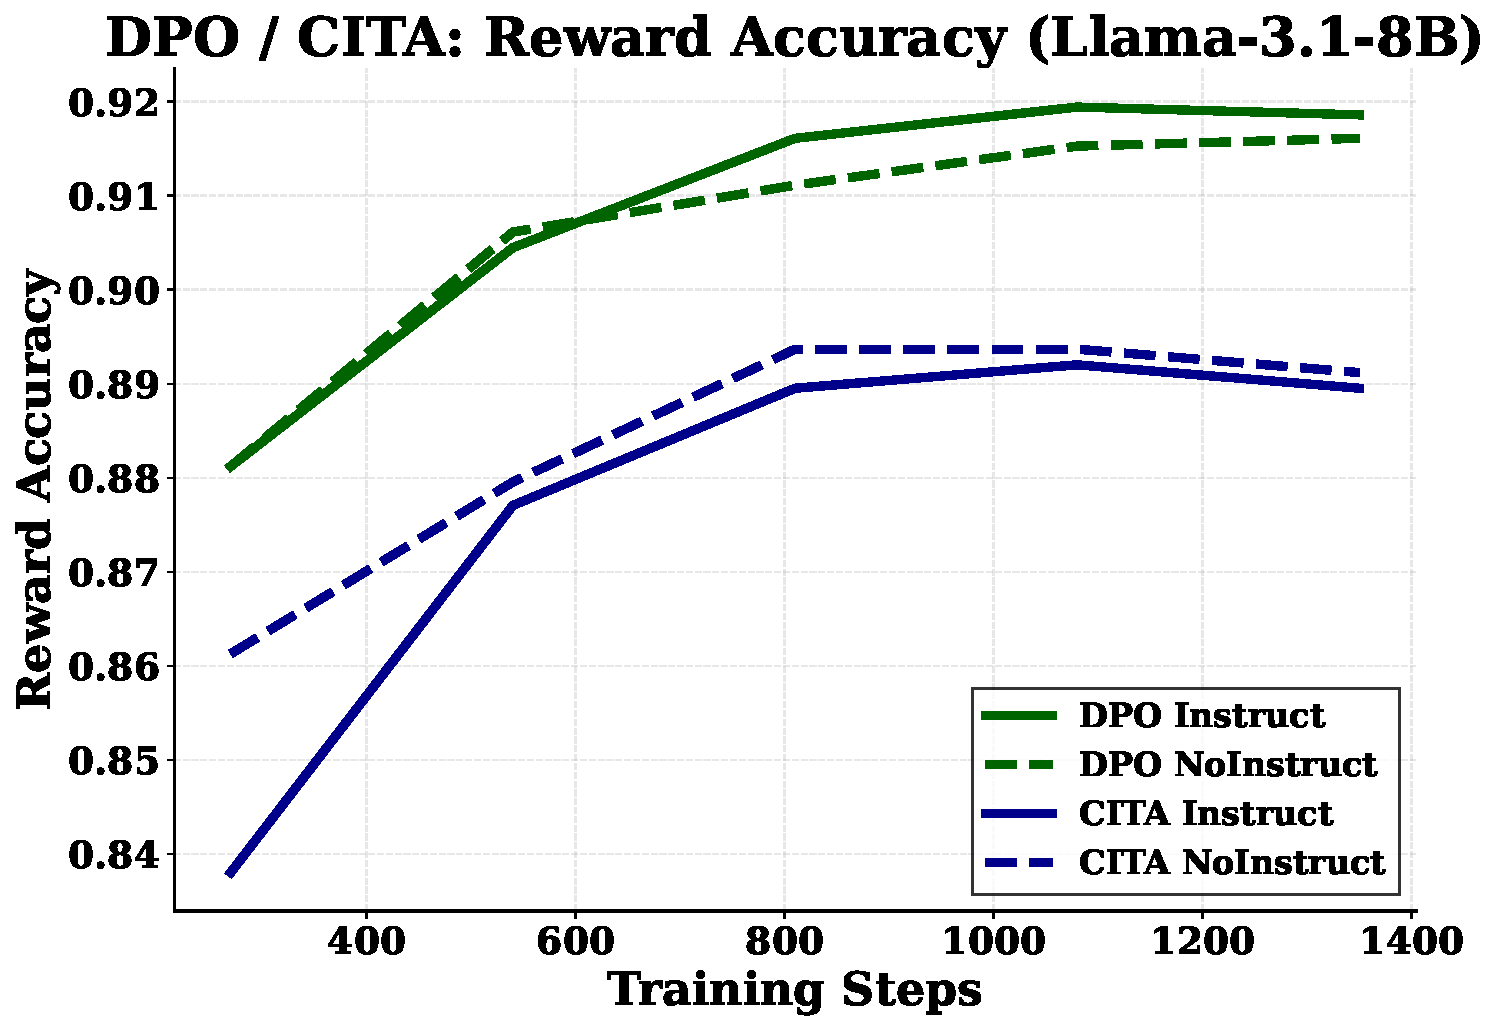
\includegraphics[width=0.9\textwidth]{figures/training/combined_accuracy.pdf}
\caption{\textbf{Training Accuracy Metrics}: 1$\times$2 subplot comparing accuracy across methods. \textbf{Left (DPO/CITA)}: Reward accuracy---all models converge to 89--92\%, with DPO variants achieving slightly higher accuracy. \textbf{Right (SFT)}: Mean token accuracy---both variants converge smoothly, with Instruct achieving marginally higher accuracy due to richer training signal from instruction-augmented sequences.}
\label{fig:training_accuracy}
\vspace{-3mm}
\end{figure*}

\begin{figure}[H]
\centering

\includegraphics[width=0.9\columnwidth]{figures/training/dpo_cita_margins.pdf}
\caption{\textbf{Reward Margins}: CITA\_Instruct (7.5) $>$ CITA\_NoInstruct (7.1) $>$ DPO ($\sim$6.0). Higher margins indicate stronger preference learning.}
\label{fig:training_margins}
\vspace{-3mm}
\end{figure}

\textbf{Key Observation.} CITA achieves higher reward margins (7.5 vs. 6.0) than DPO despite similar accuracy, validating that mandatory KL regularization leads to stronger preference differentiation.
